%
%  untitled
%
%  Created by Colin Williams on 2012-01-06.
%  Copyright (c) 2012 __MyCompanyName__. All rights reserved.
%
\documentclass[]{article}

% Use utf-8 encoding for foreign characters
\usepackage[utf8]{inputenc}

% Setup for fullpage use
\usepackage{fullpage}

% Uncomment some of the following if you use the features
%
% Running Headers and footers
%\usepackage{fancyhdr}

% Multipart figures
%\usepackage{subfigure}

% More symbols
%\usepackage{amsmath}
%\usepackage{amssymb}
%\usepackage{latexsym}

% Surround parts of graphics with box
\usepackage{boxedminipage}

% Package for including code in the document
\usepackage{listings}

% If you want to generate a toc for each chapter (use with book)
\usepackage{minitoc}

% This is now the recommended way for checking for PDFLaTeX:
\usepackage{ifpdf}
\usepackage{comment}

%\newif\ifpdf
%\ifx\pdfoutput\undefined
%\pdffalse % we are not running PDFLaTeX
%\else
%\pdfoutput=1 % we are running PDFLaTeX
%\pdftrue
%\fi


\usepackage{array}
\usepackage{url}
\usepackage{listings}
\usepackage{color}
\usepackage{amsmath}
\usepackage{mathtools}

\definecolor{dkgreen}{rgb}{0,0.6,0}
\definecolor{gray}{rgb}{0.5,0.5,0.5}
\definecolor{mauve}{rgb}{0.58,0,0.82}

\lstset{
  language=Java,
  tabsize=4,
  showstringspaces=false,
  basicstyle=\tt,
  numberstyle=\tiny\color{gray},      % line number style
  keywordstyle=\color{blue},          % keyword style
  commentstyle=\color{dkgreen},       % comment style
  stringstyle=\color{mauve},          % string literal style
}

\ifpdf
\usepackage[pdftex]{graphicx}
\else
\usepackage{graphicx}
\fi
\title{Negotiation User Guide}
\author{T. Baarslag, W. Pasman, K. Hindriks, D. Tykhonov, W. Visser, M. Hendrikx}

\date{\today}

% Alter some LaTeX defaults for better treatment of figures:
    % See p.105 of "TeX Unbound" for suggested values.
    % See pp. 199-200 of Lamport's "LaTeX" book for details.
    %   General parameters, for ALL pages:
    \renewcommand{\topfraction}{0.9}	% max fraction of floats at top
    \renewcommand{\bottomfraction}{0.8}	% max fraction of floats at bottom
    %   Parameters for TEXT pages (not float pages):
    \setcounter{topnumber}{2}
    \setcounter{bottomnumber}{2}
    \setcounter{totalnumber}{4}     % 2 may work better
    \setcounter{dbltopnumber}{2}    % for 2-column pages
    \renewcommand{\dbltopfraction}{0.9}	% fit big float above 2-col. text
    \renewcommand{\textfraction}{0.07}	% allow minimal text w. figs
    %   Parameters for FLOAT pages (not text pages):
    \renewcommand{\floatpagefraction}{0.7}	% require fuller float pages
	% N.B.: floatpagefraction MUST be less than topfraction !!
    \renewcommand{\dblfloatpagefraction}{0.7}	% require fuller float pages

	% remember to use [htp] or [htpb] for placement
	
\begin{document}

\ifpdf
\DeclareGraphicsExtensions{.pdf, .jpg, .tif}
\else
\DeclareGraphicsExtensions{.eps, .jpg}
\fi

\maketitle

\newcommand\Genius{{\sc Genius}}

\abstract{\noindent In \Genius, you can implement and analyze an agent that negotiates on your behalf. This document describes how you can install the required environment, work with the provided agents, and write, compile, and run such an agent yourself.}

\pagebreak
\tableofcontents

\pagebreak
\section{Theory Crash Course}
This section provides a crash course on some essential theory needed to understand the negotiation system. Furthermore, it provides an overview of the features of a negotiation implemented in \Genius.

\subsection{Negotiation Protocol}
The negotiation protocol determines the overall order of actions during a negotiation. Agents are obliged to stick to this protocol, and deviations from the protocol are caught and penalized. This section discusses the details of the bilateral alternating offers protocol used in \Genius.

In the bilateral alternating offers protocol two parties -- agent $A$ and agent $B$ -- take turns. Agent $A$ starts the negotiation. Each turn an agent presents one of the three possible actions:

\begin{center}
\begin{tabular}{cm{0.6\textwidth}}
\hline
\textsc{Accept} & This action indicates that agent accepts the opponent's last bid.\\
\hline
\textsc{Offer} & This action represents the bid made by an agent.\\
\hline
\textsc{EndNegotiation} & This action indicates that the agent terminates the negotiation.\\
\hline
\end{tabular}
\end{center}

When it is an agent's turn, it is informed about the opponent's action. Based on the opponent's action the agent comes up with a action, which it presents to the opponent. This process goes on until the negotiation finishes in one of the following ways:
\begin{itemize}
	\item An agent accepts the opponent's offer using the action \textsc{Accept}. The utility of the opponent's last bid is determined in the utility spaces of agent $A$ and $B$. The opponent is informed of this action via the ReceiveMessage method.
	\item The action returned is an \textsc{EndNegotiation}, which may be presented by an agent -- in which case it means that the agent walks away -- or when the deadline has passed. The score of both agents is set to their reservation value.
	\item Finally, if an agent does not follow this protocol -- for instance by sending another action that is not one of the above or by crashing -- the agents will also get their reservation values.
\end{itemize}
 
\subsection{Reservation Value}
A reservation value is a real-valued constant that sets a threshold below which a rational agent should not accept any offers. Intuitively, a reservation value is the utility associated with the Best Alternative to a Negotiated Agreement (BATNA).

A reservation value is the utility that an agent will obtain if no agreement is realized in a negotiation session. This can happen either if a an agent leaves the negotiation, or by not reaching an agreement before the deadline. In other words: either the negotiating parties agree on an outcome $\omega$, and both agents receive the associated utility of $\omega$, or: no agreement is reached, and both agents receive their reservation value instead.

Reservation values typically are different for each of the negotiating agents that negotiate in a session. In case no reservation value is set in a profile, it is assumed 0.


\subsection{Time Pressure}
A negotiation lasts a predefined time in seconds, or alternatively rounds. The time line is \emph{normalized}, i.e.: time $t \in [0, 1]$, where $t = 0$ represents the start of the negotiation and $t = 1$ represents the deadline. Notice that manipulation of the remaining time can be a factor influencing the negotiation results.

There is an important difference between a time-based and rounds-based protocol. In a time-based protocol the computational cost of an agent should be taken into account as it directly influences the amount of bids which can be made. In contrast, for a rounds-based negotiation the time can be thought of as frozen inside a round; therefore computational cost does not play a role.

Apart from a deadline, a scenario may also have \emph{discount factors}. Discount factors decrease the utility of the bids under negotiation as time passes. Time is shared between the agents, but the discount is private too, and can different for each agent. The implementation of discount factors is as follows: let $d$ in $[0, 1]$ be the discount factor that is specified in the preference profile of an agent; let $t$ in $[0, 1]$ be the current normalized time, as defined by the timeline; we compute the discounted utility $U_D^t$ of an outcome $\omega$ from the undiscounted utility function $U$ as follows:
\begin{eqnarray}
U_D^t(\omega) = U(\omega) \cdot d^t
\end{eqnarray}
If $d = 1$, the utility is not affected by time, and such a scenario is considered to be undiscounted, while if $d$ is very small there is high pressure on the agents to reach an agreement. Note that discount factors are part of the preference profiles and therefore different agents may have a different discount factor.

If a discount factor is present, reservation values will be discounted in exactly the same way as the utility of any other outcome. It is worth noting that, by having a discounted reserve price, it may be rational for an agent to end the negotiation early and thereby default to the reservation value.

\subsection{Negotiation Objects}
Agent participating in a negotiation interact in a scenario. A scenario specifies the possible bids by using the domain, and the preferences for each agent with a utility space for each agent. Figure~\ref{Fig:overviewStructures} provides an overview of the relation between the domain and the utility space of an agent.

\begin{figure}[htb]
	\centering
	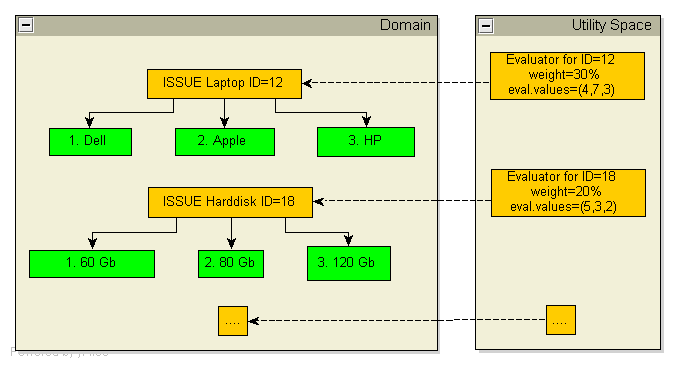
\includegraphics[width=0.5\textwidth]{media/datastructures.png}
	\caption{Overview of the data structures and relations.}\label{Fig:overviewStructures}
\end{figure}

The {\bf Domain} describes which issues are the subject of the negotiation and which values an issue can attain. To give a concrete example of a domain: in the laptop domain the issues are ``laptop'', ``harddisk'' and ``monitor''. The domain also describes the possible values that all the issues can take. In the laptop domain, the issues can only attain discrete values from a finite set, e.g. the ``harddisk'' issue can only have the values ``60 Gb'', ``80 Gb'' and ``120 Gb''. These issues are all instance of \textbf{IssueDiscrete}. There are other types of Issue, but discussion of them falls out of the scope of this short discussion.

Combining these concepts, an agent can formulate a \textbf{Bid}: a mapping from each issue to a value. A valid bid in the laptop domain is for example a Dell laptop with 80 Gb and a 17' inch monitor.

The {\bf UtilitySpace} specifies the preferences of the bids for an agent. Using a utility space the utility of a bid can be calculated. The utility is calculated using evaluators. Each issue has an evaluator corresponding to the type of the issue. The evaluator maps the evaluation of a value of an issue -- which is specified in the preference profile -- to a utility for that issue. The evaluator also specifies the importance of the issue relative to the other issues in the form of a weight. The weights of all issues sum up to 1.0. To illustrate, the ``harddisk'' issue is of the type \textbf{IssueDiscrete}, and therefore its evaluator is of the type \textbf{EvaluatorDiscrete}.

In general, given the set of all bids, there are a small subset of bids which are more preferred as outcomes by both agents. Identifying these special bids may lead to a better agreement for both parties. We discuss the optimality of a bid in the next section.

\subsection{Optimality of a Bid}
Before discussing the optimality of a bid, we first need to formalize the concept of a bid. A bid is a set of chosen values $v_1, \ldots, v_n$  for each of the $N$ issues. Each of these values has been assigned an evaluation value $\text{eval}(v_i)$ in the utility space. The utility is the weighted sum of the normalized evaluation values.

\begin{equation}
	U(v_1, \ldots, v_n) = \sum_{i=1}^{N} w_i \dfrac{\text{eval}(v_i)}{\text{max}(\text{eval}(v_i))}
	\label{eqn:Utility}
\end{equation}

For a single agent, the optimal bid is of maximum utility for the agent. Often this bid has a low utility for the opponent, and therefore the chance of agreement is low. A more general notion of optimality of a negotiation involves the utility of both agents. Figure~\ref{Fig:utility plot} shows the utilities of all bids for both parties.
 
\begin{figure}[htb]
	\centering
	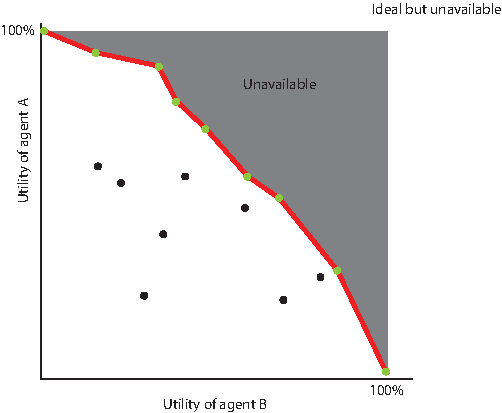
\includegraphics[width=0.4\textwidth]{media/image5.pdf}
\caption{A point indicates the utility for both agents of a bid. The red line is the Pareto optimal frontier.}\label{Fig:utility plot}
\end{figure}

There are multiple ways to define a more global ``optimum''. One approach to optimality is that a bid is not optimal for both parties if there is another bid that has the higher utility for one party, and at least equal utility for the other party. Thus, only bids in Figure 2 for which there is no other bid at the top right is optimal. This type of optimality is called Pareto optimality and forms an important concept in automated negotiation. The collection of Pareto optimal bids is called the Pareto optimal frontier.

The challenge in an actual negotiation, is that the opponent in the default negotiation protocol hides its preference profile. This entails that an agent does not know how much the opponent prefers a bid. This problem can be partly resolved by building a model of the opponent's preferences by analyzing the negotiation trace. Each turn the agent can now offer the best bid for the opponent given a set of similar preferred bids for itself. By default, there are already a few opponent models implemented in \Genius, such as the \textbf{HardHeadedFrequencyModel} used by the HardHeaded agent which won the ANAC2011.
 
\section{Installing the Environment}
The negotiation environment has been tested extensively on Microsoft Windows. It should run on any machine running Java 6 or higher. This includes Solaris and Linux distributions. There are known issues with Linux (in particular Ubuntu and SUSE) mainly involving the visualization of the GUI. There are still a number of known bugs in the negotiation environment, but these should be non critical. Please report any bugs found to \url{ai@mmi.tudelft.nl}.

To install the environment, the file \texttt{negotiator.zip} can be downloaded. Unzip the file at a convenient location on your machine. This will result in a package containing the following files:

\begin{itemize}
	\item \texttt{userguide.pdf}, this document;
	\item \texttt{negosimulator.jar}, the negotiation simulator;
	\item a \texttt{templates} folder, containing various scenarios.
\end{itemize}

When you run the negosimulator (by double-clicking the application), progress messages and error messages are printed mainly to the standard output. On Mac OSX you can view these messages by opening the console window (double-click on Systemdisk/Applications/Utilities/Console.app). On Windows this is not directly possible. Console output can be read only if you start the application from the console window by hand, as follows. Go to the directory with the negosimulator and enter
\texttt{java -jar negosimulator.jar}
This will start the simulator, and all messages will appear in the console window. You may see some errors and warnings that are non-critical.

\section{Scenario Creation}
A negotiation can be modeled in \Genius~by creating a scenario. A scenario consists of a domain specifying the possible bids and a set of preference profiles corresponding to the preferences of the bids in the domain. This section discusses how to create a domain and a preference profile.

\subsection{Basic GUI Components}
Start \Genius~by following the instructions in the previous section. After starting the simulator a screen similar to Figure~\ref{Fig:negosimulator start} is shown. This screen is divided in three portions:

\begin{itemize}
	\item The \textbf{Menubar} (blue border) allows us to start a new negotiation.
	\item The \textbf{Components Window} (red border) shows all available scenarios and agents.
	\item The \textbf{Status Window} (green border) shows the status of the negotiation or structure of a selected domain or preference profile.
\end{itemize}

\begin{figure}[htb]
	\centering
	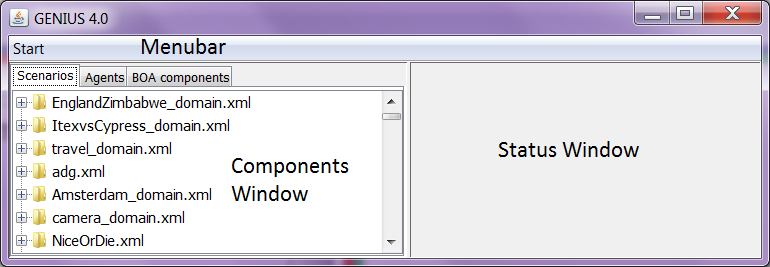
\includegraphics[width=0.6\textwidth]{media/image6.png}
\caption{The negosimulator right after start-up.}\label{Fig:negosimulator start}
\end{figure}

\subsection{Creatingyy a Domain}
By right clicking on the list of available scenarios in the Components Window a popup menu with the option to create a new domain is shown. After clicking this option it is requested where the domain should be saved. As a domain is accompanied by a set of preference profiles, it is recommended to save the file in a new directory in the templates folder. After saving the domain a window similar to Figure~\ref{Fig:newdomain} is shown. Initially, a domain contains zero issues. We can simply add an issue by pressing the ``Add issue'' button. This results in the opening of a dialog similar to Figure~\ref{fig:createIssueD}.

\begin{figure}[htb]
	\centering
	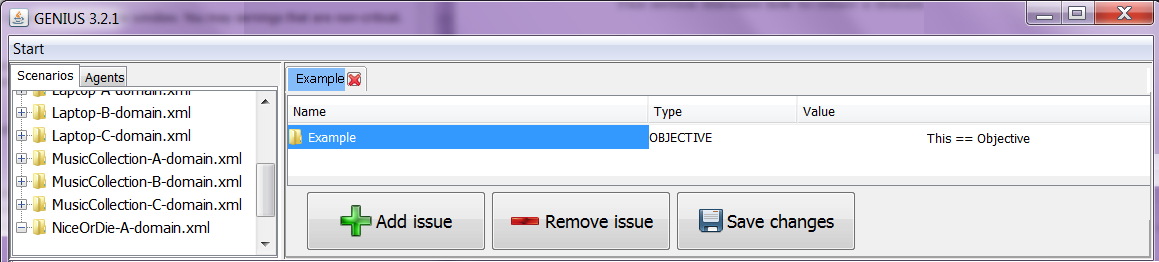
\includegraphics[width=0.7\textwidth]{media/image7.png}
\caption{The negosimulator after loading the laptop domain.}\label{Fig:newdomain}
\end{figure}

The current version of \Genius~supports the creation of discrete and integer issues. Starting with a discrete issue, the values of the issue should be specified. In Figure~\ref{fig:createIssueD} we show the values of the issue ``Harddisk''. Note the empty evaluation values window, later on when creating a preference profile we will use this tab to specify the preference of each value.

Instead of a discrete issue, we can also add an integer issue as shown in Figure~\ref{fig:createIssueI}. For an integer issue we first need to specify the lowest possible value and the highest value. Following, when creating a preference profile we need to specify the utility of the lowest value and the highest value. During the negotiation we can offer any value for the issue within the specified range.

The next step is to press ``Ok'' to add the issue. Generally, a domain consists of multiple issues. We can simply add the other issues by repeating the process above. If you are satisfied with the domain, you can save it by pressing  ``Saving changes''.

Finally, note that issues can only be added and removed when there are not yet preference profiles. This is to avoid inconsistencies between the preference profiles and the domains.

\begin{figure}[ht]
\begin{minipage}[b]{0.45\linewidth}
\centering
	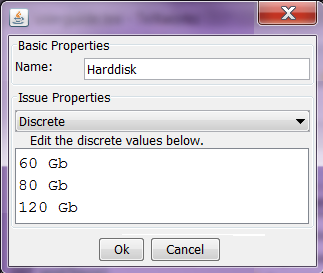
\includegraphics[width=0.8\textwidth]{media/image7a.png}
\caption{Creating a discrete issue.}
\label{fig:createIssueD}
\end{minipage}
\begin{minipage}[b]{0.45\linewidth}
\centering
	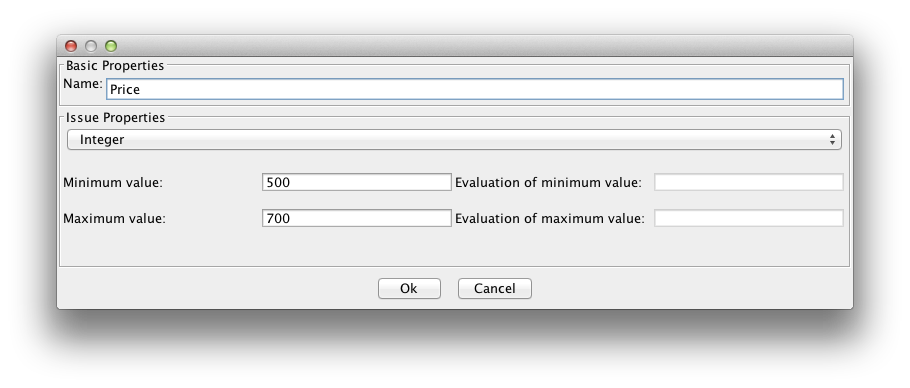
\includegraphics[width=0.8\textwidth]{media/image7b.png}
\caption{Creating an integer issue.}\label{fig:createIssueI}
\end{minipage}
\end{figure}

\subsection{Creating a Preference Profile}
Now that we created a domain, the next step is to add a set of preference profile. By right clicking on the domain a popup menu is opened which has an option to create a new preference profile. Selecting this option results in the opening of a new window which looks similar to Figure~\ref{fig:utilcreated}. It should be noted that when a domain has one or more preference profiles the issues can no longer be modified.

\begin{figure}[htb]
	\centering
	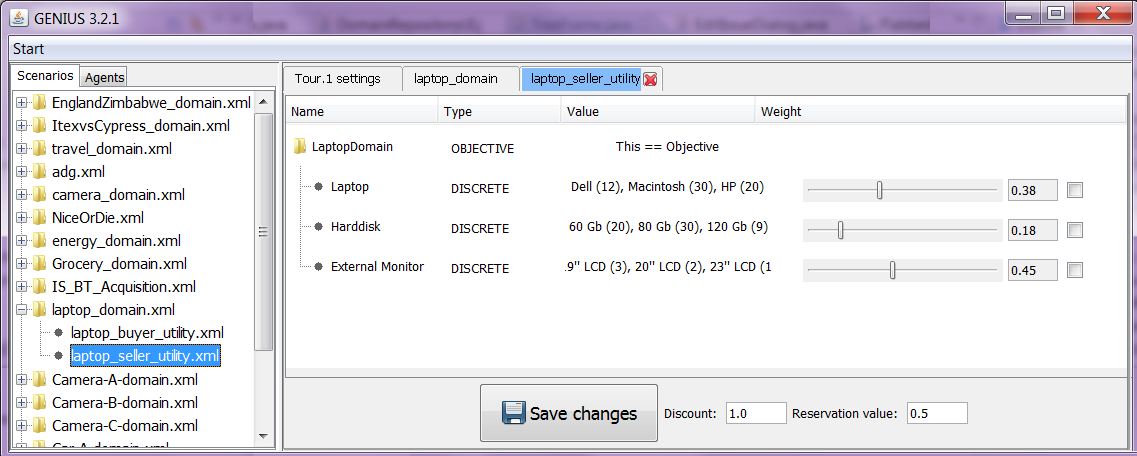
\includegraphics[width=0.8\textwidth]{media/image8.png}
\caption{The negosimulator after creating a new utility space.}\label{fig:utilcreated}
\end{figure}

Now you are ready to start customizing your utility space to reflect your personal preferences. There are two steps: setting the importance of the issues and setting the preference of the values of the issues. To start with the first step, you can adjust the relative weights of the issues by using the sliders next to that issue. Note that when you slide a slider, the weights of the other sliders are automatically updated such that the all weights still sum up to one. If you do not want this behavior, you can lock the weight of an issue by selecting the checkbox behind it.

Now that we determined the weights of the issues, it is a good idea to save the utility space by selecting ``Save changes''. The next and final step is to set the evaluation of the issues. To specify the evaluation of an issue you can double click it to open a new window looking similar to Figure~\ref{fig:createIssueD} or Figure~\ref{fig:createIssueI} depending on the type of the issue.

For a discrete issue we need to specify the evaluation value of each discrete value. A specific value can be assigned any positive non-zero integer as evaluation value. During the negotiation the utility of value is determined by dividing the value by the highest value for that particular issue. To illustrate, if we give 60 Gb evaluation 5, 80 Gb evaluation 8, and 120 Gb evaluation 10; then the utilities of these values are respectively 0.5, 0.8, and 1.0.

Specifying the preference of a integer issue is even easier. In this case we simply need to specify the utility of the lowest possible value for that issue and the utility of the highest possible value. The utility of a value in this range is calculated during the negotiation by using linear interpolation of the utilities of both given utilities. If you are satisfied with the profile you can save it by pressing ``Save changes''. 

\section{Running Negotiations}
This section discusses how to run a negotiation. There are three main modes to run a negotiation:

\begin{itemize}
	\item \textbf{Negotiation session}. A negotiation session concerns a single negotiation in which two agents compete. This mode is mainly intended for new users.
	\item \textbf{Tournament}. A tournament is a collection of sessions. Two sets of agents compete against each other on a set of domains. The results of the matches are stored in the ``log'' directory. These results can be more easily viewed by importing them into Excel and using pivot tables.
	\item \textbf{Distributed tournament}. A distributed tournament is a tournament which is stored in a database and can therefore be divided among multiple computers to speed up calculation.
\end{itemize}

Before going into detail on how each of these modes work, we first discuss the two types of agents which can be used: automated agents and non-automated agents. Automated agents are agents which can compete against other agents in a negotiation without relying on input by a user. In general, these agents are able to make a large amount of bids in a limited amount of time.

In contrast, non-automated agents are agents that are fully controlled by the user. These types of agents ask the user each round which action they should make. \Genius~by default includes the UIAgent -- which has a simple user interface -- and the more extensive Extended UIAgent.


\subsection{Running a Negotiation Session}
To run a negotiation session select ``Start'' and then ``Negotiation Session''. This opens a window similar to Figure~\ref{Fig:session}. The following parameters need to be specified to run a negotiationS:
\begin{itemize}
	\item \textbf{Negotiation protocol}. The set of available protocols. Normally ``Alternating Offers'' is used.
	\item \textbf{Side A/Side B}. The configuration of both agents which negotiate against each other.
	\item \textbf{Preference profile}. The preference profile to be used by the agent of that side.
	\item \textbf{Agent name}. The agent which should participate in the negotiation.
\end{itemize}

\begin{figure}[htb]
	\centering
	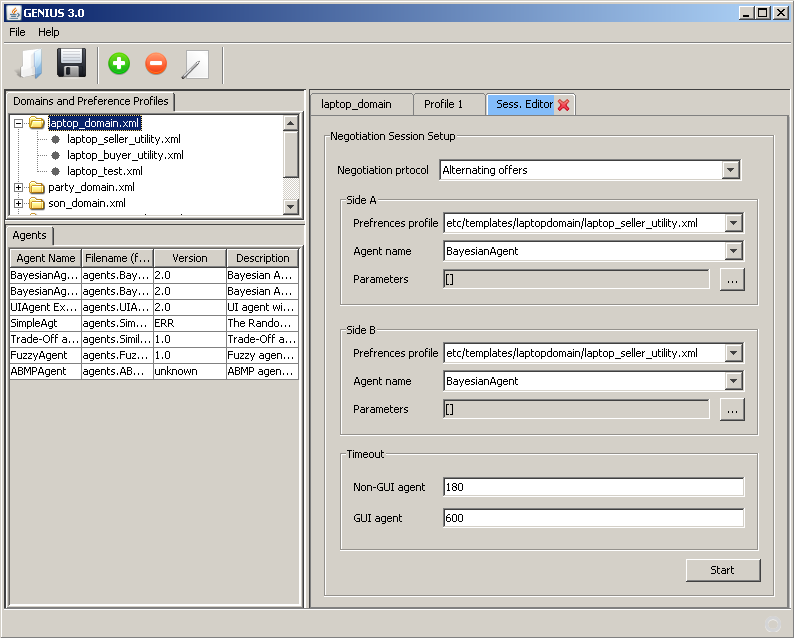
\includegraphics[width=0.6\textwidth]{media/image11.png}
\caption{A negotiation session.}\label{Fig:session}
\end{figure}


\subsection{Running a Tournament}
Besides running a single negotiation session, it is also possible to run a tournament. A tournament can be seen as a collection of sessions. In contrast to running a single session, the results of a tournament are stored in the ``log'' directory. These results can be easily analyzed by importing them into Excel an using pivot tables. A tournament can be created by first selecting ``Start'' and then ``Tournament''. The Tournament tab will appear similar to Figure~\ref{Fig:tournament}. This window shows a set of options which we need to specify. The value of an option can be specified by double clicking the option in the ``Values'' column.


\begin{figure}[htb]
	\centering
	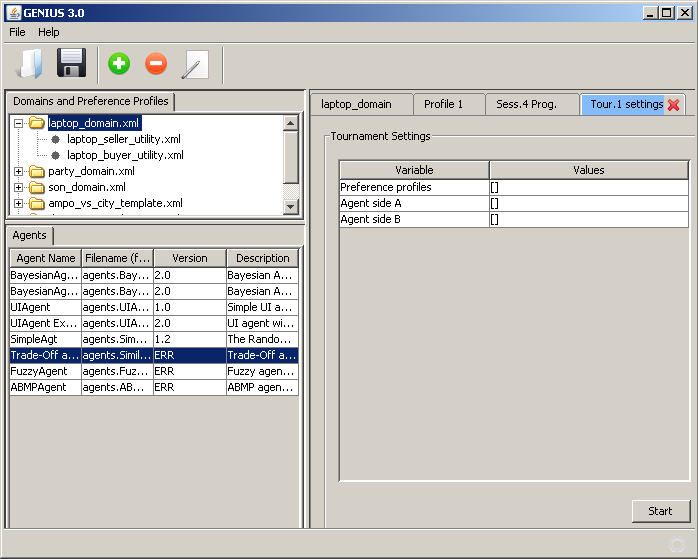
\includegraphics[width=0.8\textwidth]{media/image16.png}
\caption{Tournament tab.}\label{Fig:tournament}
\end{figure}

\begin{itemize}
	\item \textbf{Protocol}. The set of available protocols. Normally ``Alternating Offers'' is used.
	\item \textbf{Preference profiles}. The set of scenarios on which the agents should compete. Each selected scenario should feature at least two preference profiles.
	\item \textbf{Agent side A/B}. The set of agents in set A competes against all agents in set B.
	\item \textbf{Number of sessions}. The number of times each match should be repeated.
	\item \textbf{Tournament options}. Options which specify how to run the tournament (see below).
	\item \textbf{BOA Agent side A/B}. Type of agents which consist of multiple components (see~Section~\ref{sec:boa}).
\end{itemize}

In contrast to the negotiation session mode, a large set of tournament options can be specified which influence the composition and running of the tournament. There are four categories of options:
\begin{itemize}
	\item \textsc{Protocol settings}
	\begin{itemize}
		\item \textbf{Protocol mode}. Specifies if the negotiation features rounds or time. In a time-based negotiation there is an amount of time to reach an agreement. Time passes while an agent deliberates an action. In contrast, in a rounds-based negotiation the deadline is specified in rounds. An agent can take more time to compute an action as time does not pass within a round.
		\item \textbf{Deadline}. Depending on the protocol mode, this is the maximum amount of time in seconds or amount of rounds. Note that a single round corresponds to the turn of a single agent.
	\end{itemize}
	\item \textsc{Session generation}
	\begin{itemize}
		\item \textbf{Play both sides}. When generating the matches, should each pair of agents play both sides on a scenario or not.
		\item \textbf{Play against self}. An agent may be included both in the set Agent side A and side B. If this option is enabled an agent is allowed to play against itself. If disabled, the matches in which agents negotiate against themselves are removed.
	\end{itemize}
	\item \textsc{Logging}
	\begin{itemize}
		\item \textbf{Log detailed analysis}. Enabling this option activates a set of quality measures to capture the quality of the negotiation process. The quality measures are added to the default log. In addition, for the whole tournament an overview log is created. This log is prefixed with ``TM-''.
	\end{itemize}
	\item \textsc{Visualization}
	\begin{itemize}
		\item \textbf{Show all bids}. When enabled all bids in a scenario are visualized as red points in the negotiation status window. This option has a minor impact on performance.
		\item \textbf{Show last bid}. When enabled the last bid is marked with a special symbol to make it clear which move an agent performed. This has a negligible impact on performance.
		\item \textbf{Disable GUI}. When enabled most GUI elements are disabled. This speeds-up the negotiation up to a factor of 200 times. The progress of the tournament is printed to the console.
	\end{itemize}
\end{itemize}

\subsection{Running a Distributed Tournament}
A tournament quickly becomes practically too large to run. Running a distributed tournament resolves this problem as the tournament is stored in a database. Following, instances of \Genius~-- perhaps running on the same computer -- can connect to the database and process part of the tournament.

Before we can run a distributed tournament, we first need to setup a simple MySQL server which can be accessed by the computers. The installation of the database should include the ``InnoDB'' database engine. We will use this engine because it allows us to more easily remove old tournament data which we no longer need. Furthermore we recommend at least 50 Mb of free space. The required database structure can be created by using the SQL dump which can be found in the directory \textit{database}.

The next step is to specify a tournament to run. Towards this end, select ``Start'' and then ``Distributed tournament''. This opens a GUI similar to Figure~\ref{Fig:tournament}, except for the following four options:

\begin{itemize}
	\item \textbf{Database address}. The address of the database, for example \url{sql.ewi.tudelft.nl:3306/DG}.
	\item \textbf{Database user}. The username of the account for the database.
	\item \textbf{Database password}. The password of the user account for the database.
	\item \textbf{Database sessionname}. The identifier of the tournament. The identifier is needed as multiple distributed tournaments can be run at the same time.
\end{itemize}

After specifying the tournament and database parameters we can start the distributed tournament by pressing ``Start distributed tournament''. Selecting this button splits the tournament into smaller jobs which are stored in the database. The tournament is automatically started similar to a normal tournament. Now other computers can easily connect by specifying the database parameters and protocol and selecting ``Join distributed tournament''. Finally, after running the full tournament the results are sent to all computers and stored in the ``log'' directory. Figure~\ref{fig:dtournament} summarizes the process.

\begin{figure}[htb]
	\centering
	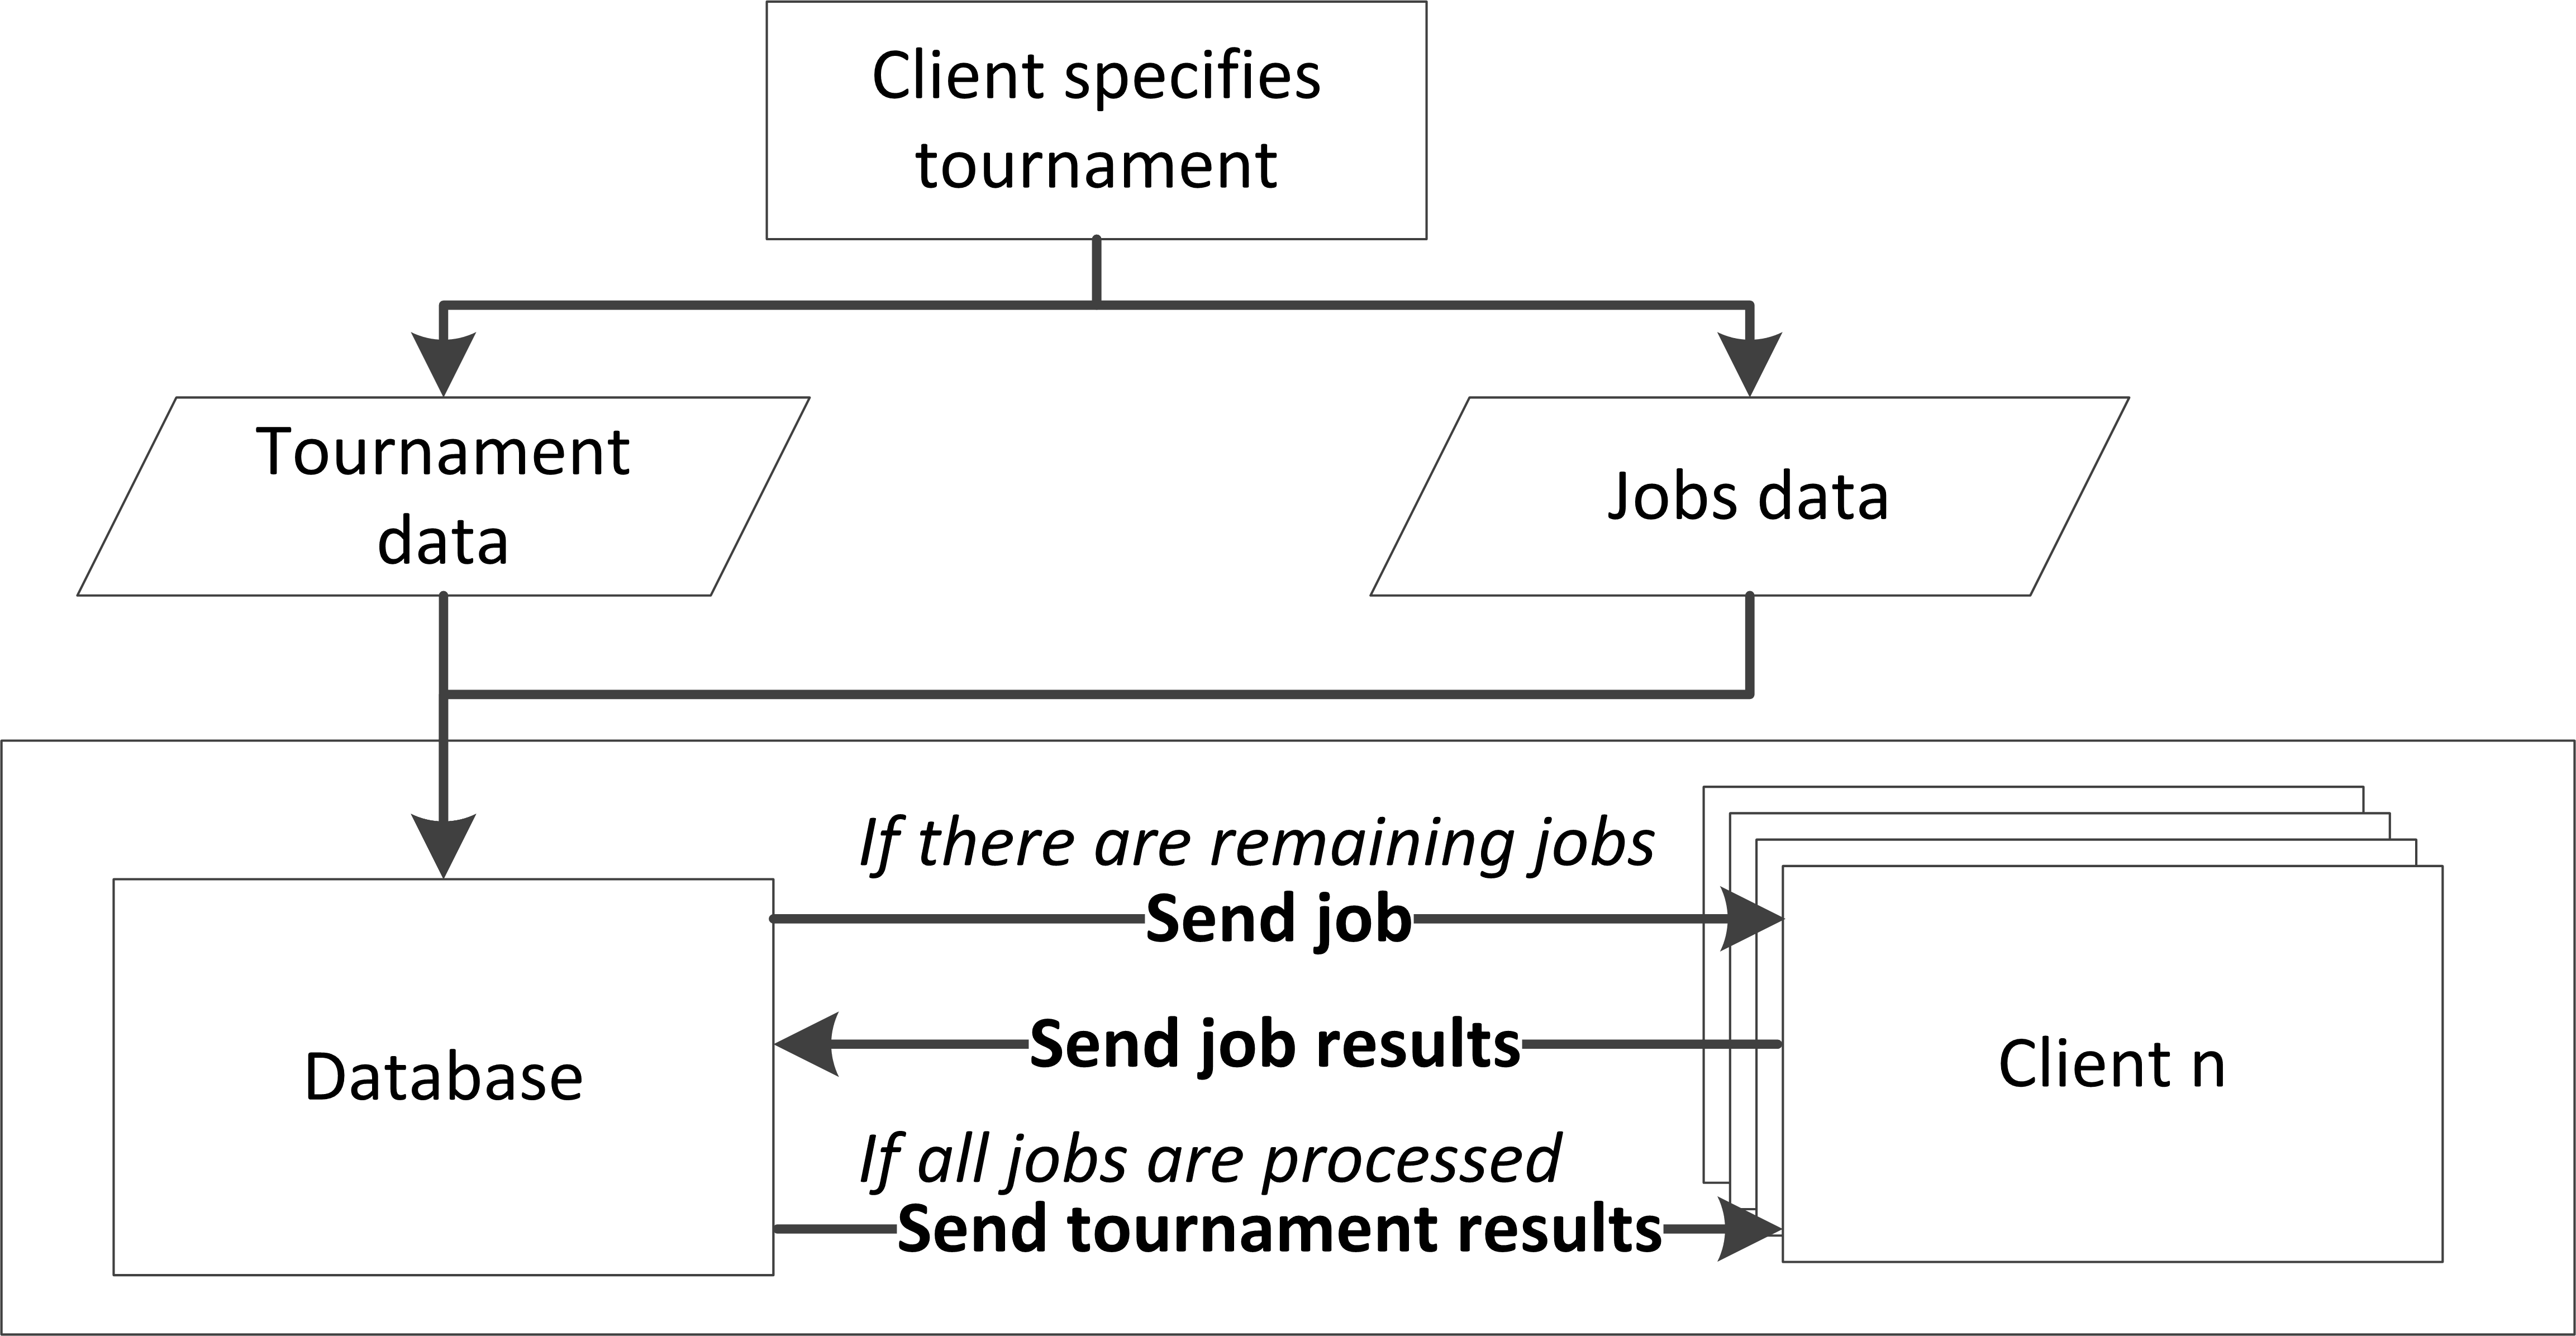
\includegraphics[width=0.50\textwidth]{media/DistributedGenius.png}
\caption{Distributed tournament process.}\label{fig:dtournament}
\end{figure}

It should be noted that currently there is no option in \Genius~to delete old tournament data. Therefore we recommend to install \textit{phpMyAdmin}. Using phpMyAdmin the old data of a tournament can be easily deleted by removing the tournament in the jobs table.

\section{Creating a Negotiation Agent}
This section discusses how to create a basic negotiation agent. A standard negotiation agent implements an agent as a single block of logic: a mix of a bidding strategy, acceptance strategy, and possibly an opponent model. In contrast, you might want to implement a BOA agent as discussed in Section~\ref{sec:boa}. The main advantage of a BOA agent is that an agent is defined as a separate implementation of a bidding strategy, acceptance, and opponent model. This entails that existing components can be reused.

In this section we assume that you are familiar with programming in Java. In case you need more information about JAVA programming, please use the following link: \url{http://docs.oracle.com/javase/tutorial/index.html}. The Java API definitions can be found on \url{http://docs.oracle.com/javase/7/docs/api/index.html}.
In the first place, a negotiation agent has to extend the negotiator.Agent class. Table 1 shows the most important fields and methods of this class. For more information, please refer to the javadoc of \Genius. To implement your agent, you have to override the three methods: ReceiveMessage, init, and chooseAction.

\begin{table}
\begin{tabular}{m{0.9\textwidth}}
\hline
\texttt{UtilitySpace utilitySpace}\\
The preference profile of the scenario.\\
\hline
\texttt{public Timeline timeline}\\
Use timeline for every time-related by using \texttt{getTime()}.\\
\hline
\texttt{public double getUtility(Bid bid)}\\
A convenience method to get the utility of a bid taking the discount factor into account.\\
\hline
\texttt{void init()}\\
Informs the agent about beginning of a new negotiation session.\\
\hline
\texttt{void ReceiveMessage(Action opponentAction)}\\
Informs the agent which action the opponent did.\\
\hline
\texttt{Action chooseAction()}\\
This function should return the action your agent wants to make next.\\
\hline
\texttt{String getName()}\\
Returns the name of the agent. Please override this to give a proper name to your agent.\\
\hline
\end{tabular}
\caption{The most important methods and fields of the Agent class.}
\end{table}

\subsection{Receiving the Opponent's Action}
The \texttt{ReceiveMessage(Action opponentAction)} informs you that the opponent just did \texttt{opponentAction}. The \texttt{opponentAction} may be null if you are the first to place a bid, or an \texttt{Offer} containing the bid of the opponent. It may also be an \texttt{Accept} or \texttt{EndNegotiation} action.
The \texttt{chooseAction()} asks you to return an \texttt{Action} to make the next step in the negotiation.

In the SimpleAgent code, the following code is available for \texttt{ReceiveMessage}. The SimpleAgent stores the opponent's action to use it when choosing an action.

\begin{lstlisting}
public void ReceiveMessage(Action opponentAction) {
	actionOfPartner = opponentAction;
}
\end{lstlisting}

\subsection{Choosing an Action}
Below show the code of the method \texttt{chooseAction} for SimpleAgent. For safety, all code was wrapped in a try-catch block, because if our code would accidentally contain a bug we still want to return a good action (failure to do so is a protocol error and results in a utility of 0.0).

The sample code works as follows. If we are the first to place a bid, we place a random bid with sufficient utility (see the .java file for the details on that). Else, we determine the probability to accept the bid, depending on the utility of the offered bid and the remaining time. Finally, we randomly accept or pose a new random bid.

While this strategy works, in general it will lead to suboptimal results as it does not take the opponent into account. More advanced agents try to model the opponent's strategy or preference profile.

\begin{lstlisting}
public Action chooseAction() {
	Action action = null;
	try { 
		if (actionOfPartner == null) {
			action = chooseRandomBidAction();
		}
		if (actionOfPartner instanceof Offer) {
			Bid partnerBid = ((Offer) actionOfPartner).getBid();
			double offeredUtilFromOpponent = getUtility(partnerBid);
			// get current time
			double time = timeline.getTime();
			action = chooseRandomBidAction();
			
			Bid myBid = ((Offer) action).getBid();
			double myOfferedUtil = getUtility(myBid);
			
			// accept under certain circumstances
			if (isAcceptable(offeredUtilFromOpponent,myOfferedUtil,time)) {
				action = new Accept(getAgentID());
			}
		}
	} catch (Exception e) { 
		e.printStackTrace();
		action = new Accept(getAgentID()); // best guess if things go wrong. 
	}
	return action;
}
\end{lstlisting}

The method \textit{isAcceptable} implements the probabilistic acceptance function$P_\text{accept}$:

\begin{equation}
	P_\text{accept} = \dfrac{u - 2ut + 2\left(t - 1 + \sqrt{(t - 1)^2 + u(2t - 1)}\right)}{2t - 1}
\end{equation}
where $u$ is the utility of the bid made by the opponent (as measured in our utility space), and $t$ is the current time as a fraction of the total available time. Figure~\ref{Fig:Paccept} shows how this function behaves depending on the utility and remaining time. Note that this function only decides if a bid is acceptable or not. More advanced acceptance strategies also use the EndNegotiation action.
\begin{figure}[htb]
	\centering
	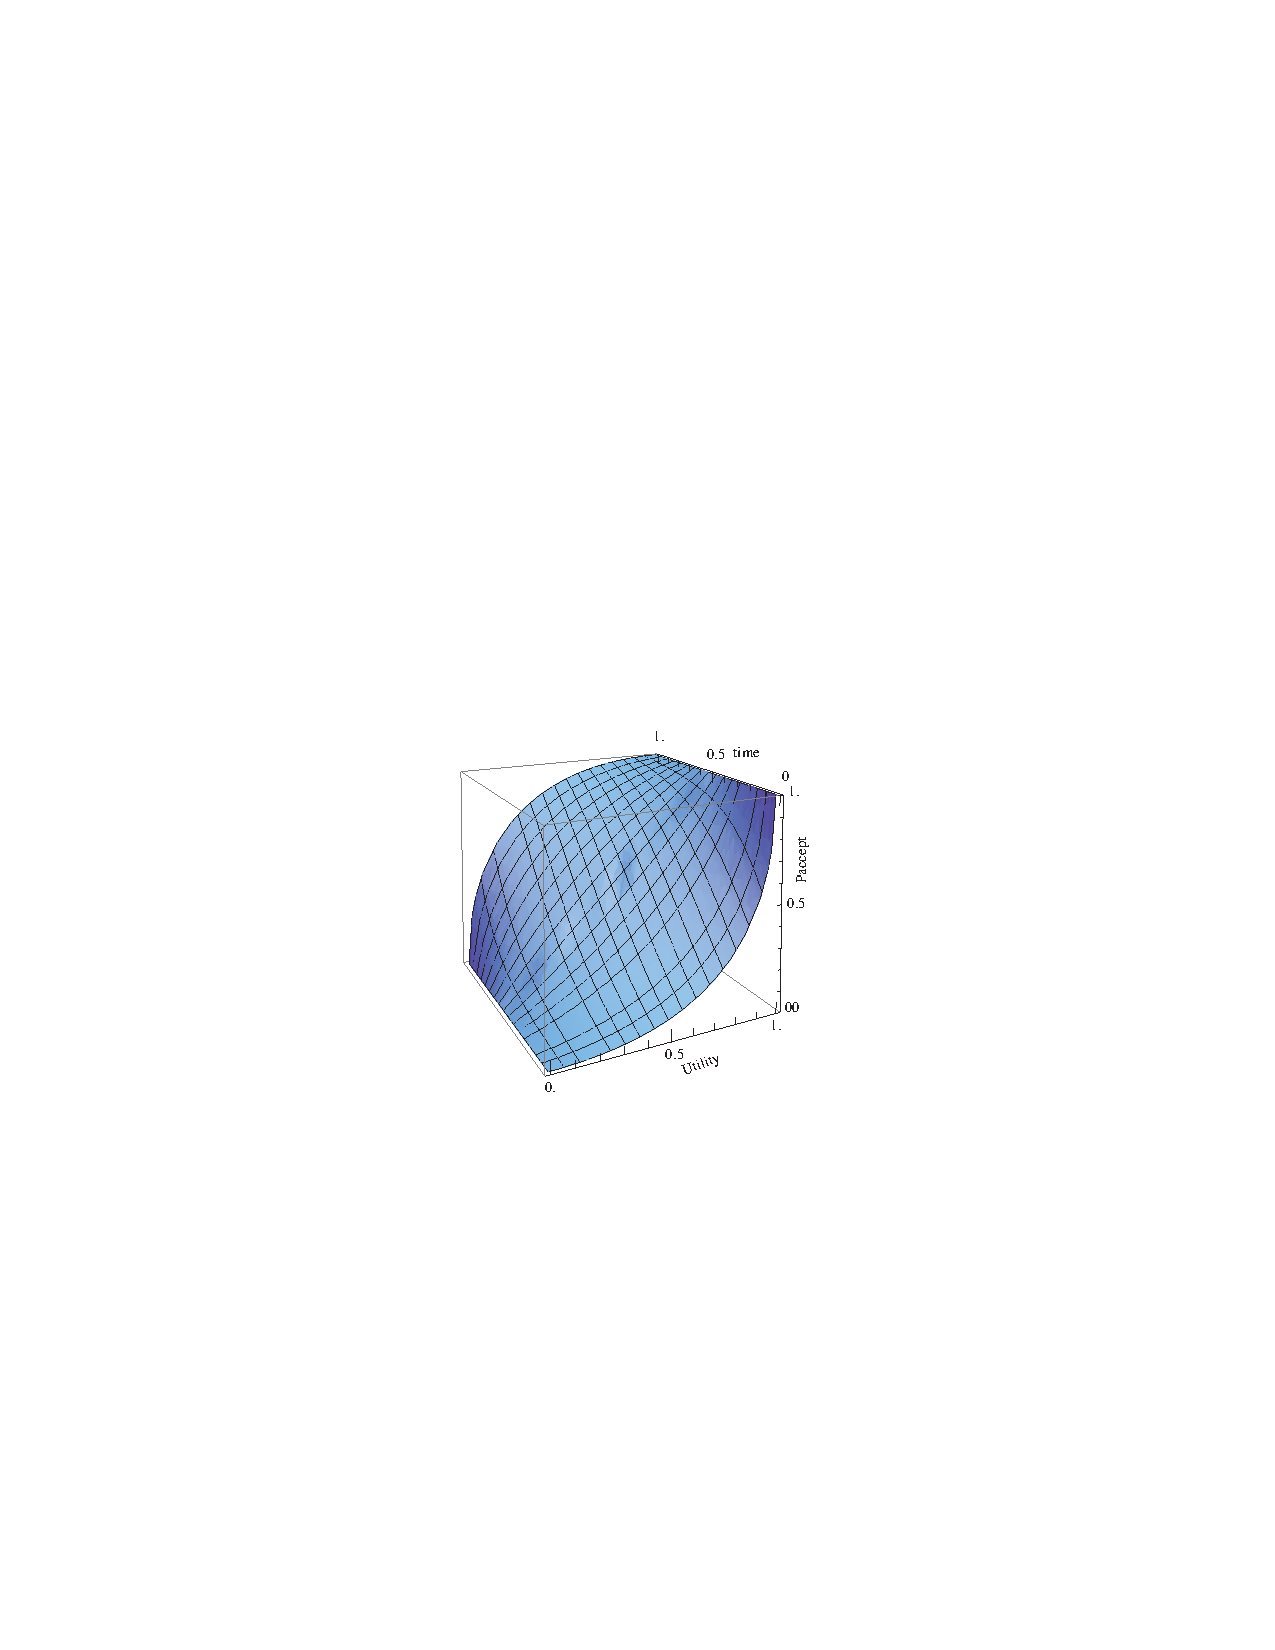
\includegraphics[width=0.3\textwidth]{media/image21.pdf}
	\caption{$P_\text{accept}$ value as function of the utility and time (as a fraction of the total available time).}\label{Fig:Paccept}
\end{figure}
%\subsection{Init}
%An important consideration for the implementation is that an agent may participate in multiple negotiation sessions with the same opponent. This enables the agent to learn from the previous sessions. For this reason, the negotiation environment calls the method \texttt{init} before starting the new session.
 
Automatic agents have to negotiate on their own, and are not allowed to communicate with a human user. Therefore, do not override the \texttt{isUIAgent()} function in automatic negotiation agents.

\subsection{Other Useful Classes}
This section provides an overview of classes which might be useful when implementing an agent.

\begin{center}
\begin{tabular}{|l|p{10.5cm}|}
\hline
\textsc{BidDetails} & Container to store a bid and its utility.\\
\hline
\textsc{BidDetailsTime} & Container to store a bid, its utility, and the time of offering.\\
\hline
\textsc{BidHistory} & Structure which can be used to keep track of the bids presented by the agent and its opponent.\\
\hline
\textsc{BidIterator} & Structure which can be used to retrieve all bids in the outcome space. It may be more interesting to use \textit{SortedOutcomeSpace}.\\
\hline
\textsc{EvaluatorDiscrete} & Evaluator which returns the utility of a value of a discrete issue. Note that this is the utility unweighted by the issue weight.\\
\hline
\textsc{EvaluatorInteger} & Evaluator which returns the utility of a value of an integer issue. Note that this is the utility unweighted by the issue weight.\\
\hline
\textsc{Issue} & Represents and issue under negotiation.\\
\hline
\textsc{IssueDiscrete} & A discrete issue.\\
\hline
\textsc{IssueInteger} & An integer issue.\\
\hline
\textsc{Pair} & A simple pair of two objects.\\
\hline
\textsc{Range} & Can be used to describe a continuous range.\\
\hline
\textsc{SortedOutcomeSpace} & Structure which stores all possible bids and their utilities. This class implements efficient search algorithms which can be used toe efficiently search the space of possible bids for bids satisfying specific properties.\\
\hline
\textsc{UtilitySpace} & Representation of a preference profile. It is recommended to use this class when implementing a model of the opponent's preference profile.\\
\hline
\end{tabular}
\end{center}

\subsection{Compiling an Agent}

To compile the agent, you put \texttt{YourAgent.java} code in the directory containing the \texttt{negotiator.jar} file, and use the command line

\texttt{javac -cp negosimulator.jar YourAgent.java}

After compilation, the resulting \texttt{YourAgent.class} file can be loaded into the negotiator simulator by typing ``YourAgent'' (fill in your actual agent name) in the negotiation set-up screen (Figure 8). Make sure your agent can be found in the same directory structure as is indicated by its package header.

\subsection{Loading an Agent with Parameters}
A compiled agent can also be loaded by directly adding the agent to the repository using the \textit{agentrepository.xml} file. The code below visualizes a repository with a single agent. An agent element consists of several subelements; the first element is the \textit{description} of the agent which is visualized in the GUI; the second element is the \textit{classPath} specifying were the compiled agent class is located; the third element specifies the \textit{agentName}; finally the optional element \textit{params} specifies the parameters and their values available to the agent. In this case, a parameter ``e'' with value 2 and a parameter ``time'' with value 0.95 is specified. Variables can be accessed during the negotiation by using the \textit{getStrategyParameters} method.

\begin{lstlisting}
<?xml version="1.0" encoding="UTF-8" standalone="yes"?>
<repository fileName="agentrepository.xml">
  <items>
   <agentRepItems>
     <agentRepItem description="Other agents - SimpleAgent"
			classPath="agents.SimpleAgent"
			agentName="SimpleAgent" params="e=2;time=0.95"/>
     </agentRepItems>
  </items>
<filename>agentrepository.xml</filename>
</repository>
\end{lstlisting}
 
ADDING AN AGENT IN THE GUI!

\section{Data structures}
For the documentation of the data structures that are relevant when writing a negotiation agent, please refer to the javadoc that can be found in your download of \Genius. 

\section{Creating a BOA Agent}\label{sec:boa}
Instead of implementing your negotiating agent from scratch, you may opt to use the \textit{BOA framework} available in \Genius: a negotiation agent architecture which allows to reuse existing components. Many of the sophisticated agent strategies that currently exist are comprised of a fixed set of modules. Generally, a distinction is made between three different modules: one module that decides whether the opponent's bid is acceptable (\textit{acceptance strategy}); one that decides which set of bids could be proposed next (\textit{bidding strategy}); and finally, one that tries to guess the opponent's preferences (\textit{opponent model}). The overall negotiation strategy is a result of the complex interaction between these components.

The advantages of separating the negotiation strategy into these three components (or equivalently, fitting an agent into the BOA framework) are threefold: first, it allows to \textit{study the performance of individual components}; second, it allows to \textit{systematically explore the space of possible negotiation strategies}; third, the identification of unique interacting components \textit{simplifies the creation of new negotiation strategies}.

\subsection{How it works}
A negotiation agent in the BOA framework, called a \textit{BOA agent}, consists of three components:
\begin{description}
  \item[Bidding strategy] A bidding strategy is a mapping which maps a negotiation trace to a bid. The bidding strategy can interact with the opponent model by consulting with it.%, passing one or multiple bids and see how they compare within the opponent's utility space.

  \item[Opponent model] An opponent model is in the BOA framework a learning technique that constructs a model of the opponent's preference profile.% In our approach, the opponent model should be able to estimate the opponent's utility of a given bid.
  \item[Acceptance strategy] The acceptance strategy determines whether the bid that the opponent has presented is acceptable.
\end{description}
The components interact in the following way (the full process is visualized in Figure~\ref{fig:flowchart}). When receiving an opponent bid, the BOA agent first updates the \textit{bidding history} and \textit{opponent model} to make sure the most up to date data is used, maximizing the information known about the environment and opponent.

Given the opponent bid, the \textit{bidding strategy} determines the counter offer by first generating a set of bids with a similar preference for the agent. The \textit{bidding strategy} uses the \textit{opponent model} (if present) to select a bid from this set by taking the opponent's utility into account.

Finally, the \textit{acceptance strategy} decides whether the opponent's action should be accepted. If the opponent's bid is not accepted by the acceptance strategy, then the bid generated by the bidding strategy is offered instead.

\begin{figure}[t] 
	\center
	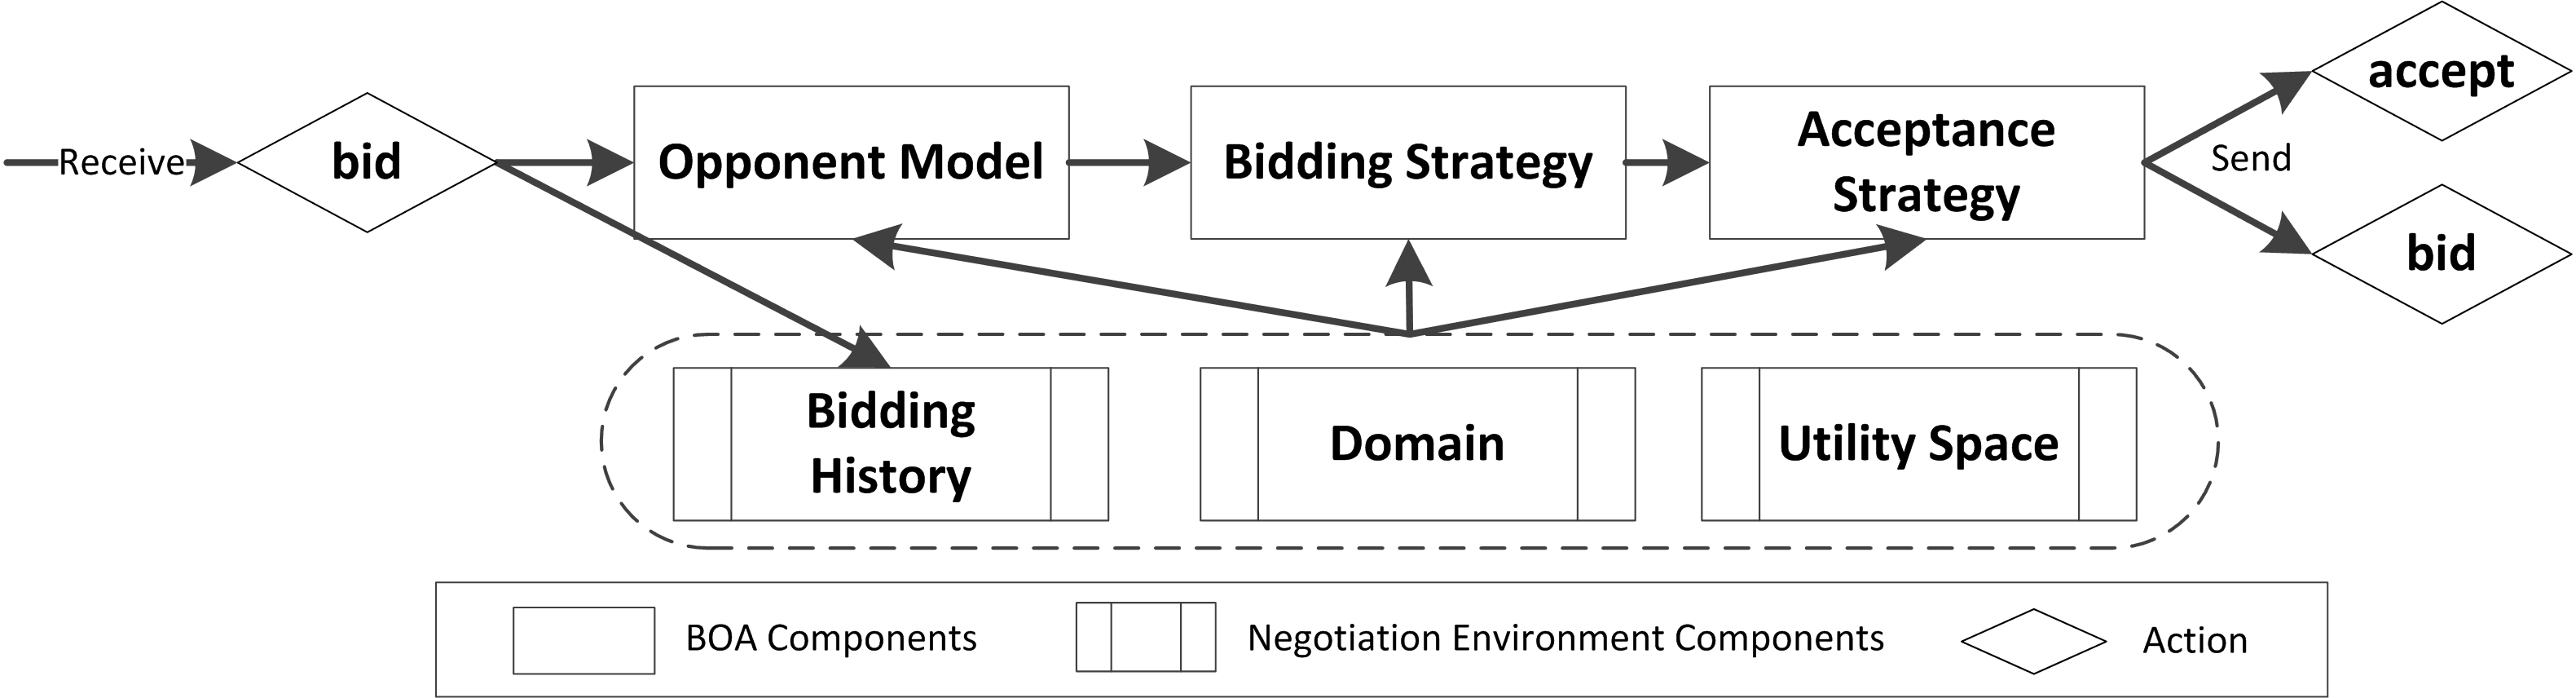
\includegraphics[width=14cm]{media/Decoupled_FlowChart.png}
	\caption{The BOA Framework Architecture.}
	\label{fig:flowchart}
\end{figure}

\subsection{Using Existing Components}
In this section we create a \textit{BOA agent} by selecting its components from a list of existing components. The first step in using the BOA framework, is to ensure it is enabled. The framework is enabled if the selected items visualized in Figure~\ref{fig:settings} are visible when creating a \textit{new tournament}.%. If the framework is not enabled, it can be enabled by changing the value of the variable \textit{DECOUPLED\_AGENTS\_ENABLED} in the \textit{Global} class located in the package \textit{negotiator}.

\begin{figure}[h!]
	\center
	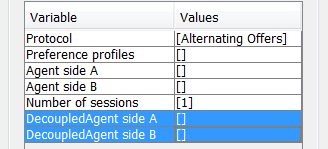
\includegraphics[width=5cm]{media/Decoupled_TournamentSettings.png}
	\caption{Tournament settings. The selected items indicate that the BOA framework is enabled.}
	\label{fig:settings}
\end{figure}

The BOA framework GUI, visualized in Figure~\ref{fig:decoupledGUI}, can be opened by clicking in the \textit{Values} section next to the \textit{BOA Agent Side A} or \textit{BOA Agent Side B}. In this GUI four component types are shown: \textit{bidding strategy}, \textit{acceptance strategy}, \textit{opponent model}, and the \textit{opponent model strategy}.

\begin{figure}[h!]
	\center
	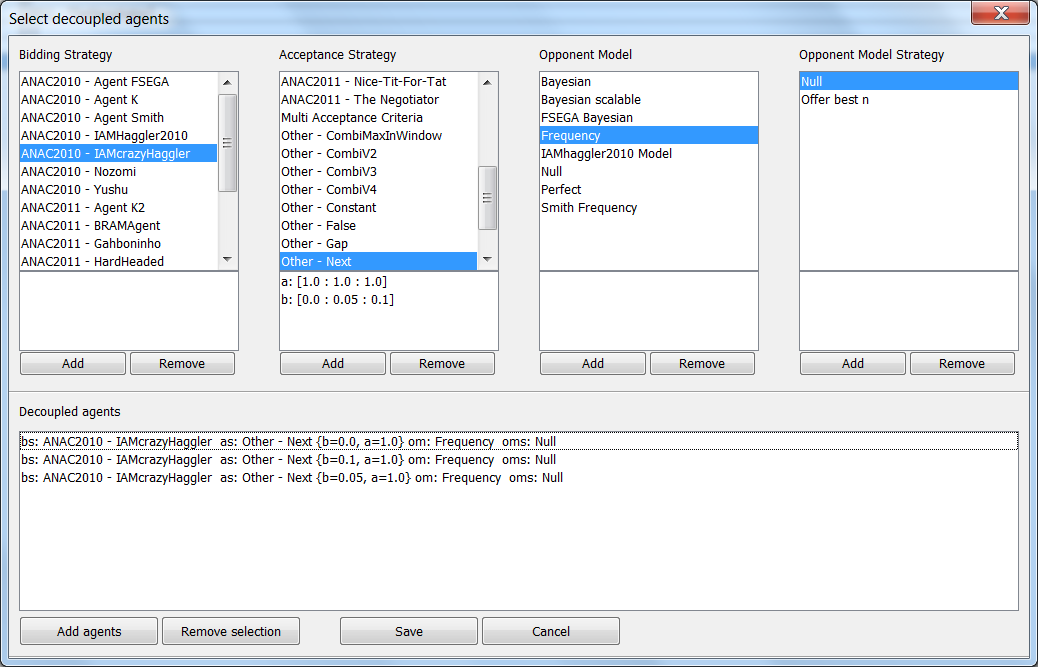
\includegraphics[width=15cm]{media/Decoupled_DecoupledGUI.png}
	\caption{The BOA framework GUI.}
	\label{fig:decoupledGUI}
\end{figure}

Our goal in this section is to create three variants of \textit{SimpleBOAagent}. First, we select the bidding strategy \textit{Other - Time Dependent} under the heading \textit{Bidding Strategy}.  If we hold our mouse still for a few seconds on this element, we see that it assumes that a parameter $e$, $k$, $max$ and $min$ are given, we will set these value to 0.2, 0, 1, 0 respectively. Parameters can be added by using the $Add$ button under each of the components (e.g. Bidding Strategy). Adding the parameter $e$ is visualized in figure~\ref{fig:decoupledparam}. Next, we select the acceptance condition \textit{Other - Next}, which expects the parameters $a$ and $b$. In our case we want to create three variants: $a=1, b=0$, $a=1, b=0.05$, and $a=1, b=0.10$. Following, we select the \textit{Frequency} opponent model. Next, we select the \textit{null} opponent model strategy. This component requires no parameters. Finally, we select ``add agents'' to create the agents and ``save'' to store them for usage in the negotiation.

\begin{figure}[h!] 
	\center
	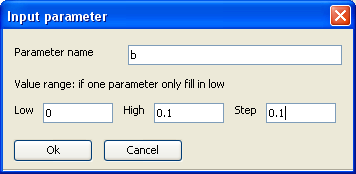
\includegraphics[width=5cm]{media/Decoupled_Param.png}
	\caption{Adding a parameter.}
	\label{fig:decoupledparam}
\end{figure}

To summarize: we created three variants of \textit{SimpleBOAagent}. All variants use a frequency opponent model, and choose a random bid out of the bids that are being considered in a round. The variants differ in when they accept, variants with a higher value for $a$ and $b$ will in general accept earlier.

\subsection{Creating New Components}
This section discusses how to create new components for the BOA framework. The next section discusses how these components can be added to the BOA framework.

\subsubsection{Creating a Bidding Strategy}
The code below is for the abstract class \textit{OfferingStrategy} which every bidding strategy needs to extend.  This class makes it compatible with the BOA framework, having it implement a \textit{init}, \textit{determineOpeningBid} and \textit{determineNextBid} methods.

The reference to \textit{negotiationsession} is important, as this object stores all information about the current match, including all bids done by the opponent and the agent itself.

The method \textit{determineOpeningBid} determines what the opening bid of the agent should be and \textit{determineNextBid} determines the counter bid the agent should offer. The variable nextBid is what the agent is planning to offer as counter bid.  This is important because there are some acceptance conditions that compares the nextBid with the offered bid of the opponent.

An approach often taken by more complex agents, is to first generate all possible bids. While this can take a long time, it allows to efficiently look up bids during the negotiation. The \textit{SortedOutcomeSpace} can be used to efficiently generate and access all possible bids during the negotiation. For an example of how to use this class we refer to the class \textit{TimeDependent\_Offering}. This class also specifies how parameters can be added.
Below is the code for the abstract class BiddingStrategy which your offering strategy should extended.

\begin{lstlisting}
public abstract class OfferingStrategy { 

	protected BidDetails nextBid;

	public void init(NegotiationSession negotiationSession, OpponentModel
						 opponentModel, OMStrategy omStrategy, 
							HashMap<String, Double> parameters)
								 throws Exception {

		this.negotiationSession = negotiationSession;
		this.opponentModel = opponentModel;
		this.omStrategy = omStrategy;
	}
	
	public abstract BidDetails determineOpeningBid();

	public abstract BidDetails determineNextBid();	
	
	public BidDetails getNextBid(){
		return nextBid;
	}
	
	public void setNextBid(BidDetails counterBid) {
		nextBid = counterBid;
	}
	
	public SharedAgentState getHelper() {
		return helper;
	}
}
\end{lstlisting}


\subsubsection{Creating an Acceptance Condition}
This section discusses the creation of an acceptance condition.  Similar to the bidding strategy the acceptance conditions needs to extend the abstract class \textit{AcceptanceStrategy} (see code below).  By extend this class the acceptance conditions should implement\textit{init} and \textit{determineAcceptability}.

The \textit{determineAcceptability} methods determines the acceptability of the offer the opponent has presented.  This method can return three actions; accept (the bid is acceptable), reject (the bid is not acceptable) and break-off (the bid is not acceptable and end the negotiation).  In some scenarios it is rational to return break-off (end the negotiation prematurely) for example if one is working with reservation values.

\begin{lstlisting}
public abstract class  AcceptanceStrategy {

	public void init(NegotiationSession negotiationSession, OfferingStrategy 
						offeringStrategy, HashMap<String, Double> parameters)
							throws Exception {
	
		this.negotiationSession = negotiationSession;
		this.offeringStrategy = offeringStrategy;
	}
	
	public String printParameters(){
		return"";
	}
	
	public abstract Actions determineAcceptability();
}
\end{lstlisting}

\subsubsection{Creating an Opponent Model}
This section discusses how to create an opponent model. An opponent model in the BOA framework should extend the \textit{OpponentModel} class (see code below). This class enforces that at least \textit{init}, \textit{updateModel}, \textit{getBidEvaluation} and \textit{getDiscountedBidEvaluation} are implemented. The \textit{updateModel} is given a bid which is then used to update the opponent model.  This method should be called when a new bid is received from the opponent. The methods \textit{getBidEvaluation} and \textit{getDiscountedBidEvaluation} are used to obtain the estimated (discounted) utility of the opponent for a particular bid based on the opponent model. Since opponent models are relatively more complex to implement in comparison to the other components, we do not present an example but instead refer to the class \textit{IAMhaggler2010 Model}.\\

\begin{lstlisting}
public abstract class OpponentModel {
	
	protected NegotiationSession negotiationSession;
	protected UtilitySpace opponentUtilitySpace;
	
	public void init(NegotiationSession domainKnow, HashMap<String, Double> parameters) throws Exception {
		negotiationSession = domainKnow;
		opponentUtilitySpace = new UtilitySpace(domainKnow.getUtilitySpace());
	}
	
	public void init(NegotiationSession domainKnow) {
		negotiationSession = domainKnow;
		opponentUtilitySpace = new UtilitySpace(domainKnow.getUtilitySpace());
	}

	public abstract void updateModel(Bid opponentBid);

	public double getBidEvaluation(Bid b){
		try {
			return opponentUtilitySpace.getUtility(b);
		} catch (Exception e) {
			e.printStackTrace();
		}
		return -1;
	}
	
	public double getDiscountedBidEvaluation(Bid b, double time){
		return opponentUtilitySpace.getUtilityWithDiscount(b, time);
	}
	
	public UtilitySpace getOpponentUtilitySpace(){
		return opponentUtilitySpace;
	}

	public void setOpponentUtilitySpace(BilateralAtomicNegotiationSession fNegotiation) { }
}
\end{lstlisting}


The opponent model also comprise of a sub-component, the \textit{Opponent Model Strategy}. This component interacts closely with the bidding strategy, determining which bid the opponent model should return when presented with alternatives and when the opponent model may be updated. A opponent model strategy class should extend the \textit{OMStrategy} (see below) class and implement \textit{init}, \textit{canUpdateOM} and \textit{getBid}.

\begin{lstlisting}
package negotiator.boaframework;
public abstract class OMStrategy {
	public void init(NegotiationSession negotiationSession, OpponentModel model, HashMap<String, Double> parameters) throws Exception {
		this.negotiationSession = negotiationSession;
		this.model = model;
	}
	
	public void init(NegotiationSession negotiationSession, OpponentModel model) {
		this.negotiationSession = negotiationSession;
		this.model = model;
	}
	
	public abstract BidDetails getBid(List<BidDetails> bidsInRange);
	
	public BidDetails getBid(OutcomeSpace space, Range range) {
		List<BidDetails> bids = space.getBidsinRange(range);
		if (bids.size() == 0) {
			range.increaseUpperbound(RANGE_INCREMENT);
			if (range.getUpperbound() < 1.1) {
				return getBid(space, range);
			} else {
				negotiationSession.setOutcomeSpace(space);
				return negotiationSession.getMaxBidinDomain();
			}
		}
		return getBid(bids);
	}
	
	public abstract boolean canUpdateOM();
}
\end{lstlisting}

\subsection{Creating A BOA Agent}
There are two ways of creating a BOA agent; One is to use the component repository and select the components from the BOA framework GUI.  The other way us to create an agent class and add it to the agent repository.

\subsubsection{Adding Components to the Repository}
In the previous section we discussed how to create the components. To use the components, we still need to add them to the \textit{BOA repository}. The \textit{BOA repository} is located in the main directory of \Genius ~and its structure is similar to the small repository shown below. There are four main categories corresponding to the component types. Each element in a category has to specify a description and a classpath. Optionally, a tooltip element can be specified to discuss which parameters are expected.

\begin{lstlisting}
<?xml version="1.0" encoding="UTF-8" standalone="yes"?>
<repository fileName="boarepository.xml">
  <biddingstrategies>
  <biddingstrategy description="ANAC2010 - IAMcrazyHaggler" 
		classPath="IAMCrazyHaggler_Offering"/>
  </biddingstrategies>
  <acceptanceconditions>
  <acceptancecondition description="Other - Next" classPath="AC_Next" 
		tooltip="'a' for multiplier. 'b' for constant."/>		
  </acceptanceconditions>
  <opponentmodels>
   <opponentmodel description="IAMhaggler2010 Model" 
		classPath="IAMhagglerModel" tooltip="'t' for time. 'a' for use all bids"/>
  </opponentmodels>
  <omstrategies>
  <omstrategy description="Null" classPath="NullStrategy"/>
  </omstrategies>
</repository>
\end{lstlisting}

\subsubsection{Creating BOA Agent without Interface}
To create a BOA agent without using the GUI you have to create a class that extends BOA agent.  This allows you to still make use of the framework however not have to place it in the component repository.  Below is an example of an agent class that uses the BOA framework.  This class is very simple, where in agent setup the components need to be defined and initialized.

\begin{lstlisting}
public class SimpleBOAagent extends BOAagent{

	@Override
	public void agentSetup() {
		OpponentModel om = new FrequencyModel(negotiationSession, 0.2, 1);
		OMStrategy oms = new NullStrategy(negotiationSession);
		OfferingStrategy offering  = new TimeDependent_Offering(negotiationSession, om, oms, 0.2, 0, 1, 0); //Bouwlware agent strategy
		AcceptanceStrategy ac = new AC_Next(negotiationSession, offering, 1, 0);
		setDecoupledComponents(ac, offering, om, oms);		
	}

	@Override
	public String getName() {
		return "SimpleBOAagent";
	}

}
\end{lstlisting}

\subsection{Multi-Acceptance Criteria (MAC)}
The \textit{BOA framework} allows us to better explore a large space of negotiation strategies. MAC can be used to scale down the negotiation space, and thereby make it more computationally explorable.

As discussed in the introduction of this chapter, the acceptance condition determines solely if a bid should be accepted. This entails that it does not influence the bidding trace, except for when it is stopped. In fact, the only difference between \textit{BOA agents} where only the acceptance condition vary, is the time of agreement (assuming that the computational cost of the acceptance conditions are negligible).

Given this property, multiple acceptance criteria can be tested in parallel during the same negotiation trace. In practice, more than 50 variants of for example $\textbf{AC}_{next}$ can be tested in the same negotiation at a negligible computational cost.

To create a multi-acceptance condition component you first need to extend the class \textit{Mulit Acceptance Condition}, this gives access to the ACList which is a list of acceptance conditions to be tested in parallel. An acceptance can be added to the MAC by appending it to the AClist The code below illustrates an example of a MAC component.

\begin{lstlisting}
public class AC_MAC extends Multi_AcceptanceCondition {

	@Override
	public void init(NegotiationSession negoSession, OfferingStrategy strat, 
			HashMap<String, Double> parameters) throws Exception {
		this.negotiationSession = negoSession;
		this.offeringStrategy = strat;
		outcomes = new ArrayList<OutcomeTuple> ();
		ACList = new ArrayList<AcceptanceStrategy>();
		
		for (int e = 0; e < 5; e++) {
			ACList.add(new AC_Next(negotiationSession, offeringStrategy, 1, 
												e * 0.01));
		}
	}
}

\end{lstlisting}


%\bibliographystyle{plain}
%\bibliography{}
\end{document}
